\section{Averaged Result of Multiple Video Sequences}
\label{sec:results/section_a}

Running the experiment with all the possible combinations of QP and MSR as shown in Table \ref{tab:qp_msr_range}, we obtained the result from all the 12 video sequences or 12 samples in a statistical term. Since we have multiple video samples, we averaged each score of metrics with respect to QP and MSR. Table \ref{tab:averaged_result_all} shows mean values of each score from the different metrics over different QP and MSR. Each numerical value is a mean of 12 measured values of score. Table \ref{tab:averaged_result_all_std} shows their standard deviation values. Since each video sample differs in resolution, frame rare, number of objects and object classes, tracking performance is different. Due to the lack of video samples, the standard deviation is high among the 12 video samples. We believe that to have lower standard deviation, we need to have more video samples. As there are 20 metrics for object tracking performance and MOTA is a good indicator for the general tracking performance as explained in Chapter \ref{chap:background}, we visualized MOTA score for different QP and MSR as shown in Figure \ref{fig:averaged_result_all}. 
\begin{table}[!htbp]
  \centering
  \caption[Averaged performance results of all video samples]
  {Averaged performance results of all video samples.}

  % table for uncompressed
  \begin{subtable}[t]{\linewidth}
    \centering
    \vspace{0pt}
    \resizebox{1.0\linewidth}{!}{
    \begin{tabular}{llrrrrrrrrrrrrrrrrrrrr}
    \toprule
              QP &          MSR &    IDTP &   IDFP &    IDFN &  IDF1 &   IDP &   IDR &  Recall &  Precision &    F1 &    GT &   MT &   PT &   ML &      TP &     FP &      FN &   IDs &    FM &  MOTA &  MOTP \\
    \midrule
    Uncompressed & Uncompressed & 1762.58 & 932.83 & 2522.67 & 49.88 & 61.13 & 43.48 &   62.17 &      89.25 & 72.08 & 12.25 & 4.67 & 3.25 & 4.33 & 2249.75 & 441.67 & 2035.50 & 24.08 & 35.17 & 54.49 & 82.03 \\
    \bottomrule
    \end{tabular}}
    \caption{Mean values for the uncompressed sequence}
  \end{subtable}
 
 
 
  
  % table for msr=8
  \begin{subtable}[t]{\linewidth}
    \centering
    \resizebox{1.0\linewidth}{!}{
    \begin{tabular}{rrrrrrrrrrrrrrrrrrrrrr}
    \toprule
     QP &  MSR &    IDTP &   IDFP &    IDFN &  IDF1 &   IDP &   IDR &  Recall &  Precision &    F1 &    GT &   MT &   PT &   ML &      TP &     FP &      FN &   IDs &    FM &  MOTA &  MOTP \\
    \midrule
     18 &    8 & 1770.08 & 947.50 & 2515.17 & 50.60 & 61.55 & 44.26 &   62.18 &      88.58 & 71.92 & 12.25 & 4.50 & 3.17 & 4.58 & 2246.75 & 466.83 & 2038.50 & 24.17 & 36.00 & 53.97 & 82.11 \\
     22 &    8 & 1780.83 & 931.92 & 2504.42 & 50.46 & 61.66 & 43.96 &   61.62 &      88.85 & 71.65 & 12.25 & 4.58 & 3.17 & 4.50 & 2250.00 & 458.75 & 2035.25 & 24.92 & 35.58 & 53.70 & 82.10 \\
     26 &    8 & 1751.67 & 874.17 & 2533.58 & 50.41 & 62.63 & 43.28 &   60.49 &      89.73 & 71.22 & 12.25 & 4.33 & 3.17 & 4.75 & 2192.92 & 428.92 & 2092.33 & 24.33 & 35.50 & 53.24 & 82.28 \\
     30 &    8 & 1731.50 & 960.08 & 2553.75 & 49.88 & 62.12 & 42.65 &   60.21 &      89.83 & 71.07 & 12.25 & 4.33 & 3.08 & 4.83 & 2234.42 & 453.17 & 2050.83 & 23.67 & 35.00 & 53.13 & 82.16 \\
     34 &    8 & 1653.92 & 855.08 & 2631.33 & 48.14 & 62.23 & 39.93 &   57.12 &      90.61 & 69.26 & 12.25 & 4.08 & 3.00 & 5.17 & 2092.58 & 412.42 & 2192.67 & 21.75 & 32.25 & 50.64 & 82.42 \\
     38 &    8 & 1488.50 & 781.08 & 2796.75 & 44.56 & 61.38 & 35.62 &   52.70 &      91.52 & 65.97 & 12.25 & 3.42 & 3.17 & 5.67 & 1912.42 & 353.17 & 2372.83 & 21.92 & 30.67 & 47.15 & 82.29 \\
     42 &    8 & 1399.25 & 733.83 & 2886.00 & 40.92 & 60.67 & 32.08 &   46.86 &      91.35 & 60.24 & 12.25 & 3.08 & 3.25 & 5.92 & 1805.67 & 323.42 & 2479.58 & 20.83 & 33.50 & 41.48 & 81.42 \\
     46 &    8 & 1046.50 & 673.33 & 3238.75 & 30.48 & 57.12 & 22.40 &   33.09 &      87.46 & 45.48 & 12.25 & 1.75 & 3.08 & 7.42 & 1358.33 & 357.50 & 2926.92 & 18.00 & 28.25 & 27.64 & 80.47 \\
    \bottomrule
    \end{tabular}}
    \caption{Mean values for MSR = 8}
  \end{subtable}
 
 
  
  % table for msr=16
  \begin{subtable}[t]{\linewidth}
    \centering
    \resizebox{1.0\linewidth}{!}{
    \begin{tabular}{rrrrrrrrrrrrrrrrrrrrrr}
    \toprule
     QP &  MSR &    IDTP &   IDFP &    IDFN &  IDF1 &   IDP &   IDR &  Recall &  Precision &    F1 &    GT &   MT &   PT &   ML &      TP &     FP &      FN &   IDs &    FM &  MOTA &  MOTP \\
    \midrule
     18 &   16 & 1749.25 & 964.25 & 2536.00 & 50.48 & 61.51 & 44.07 &   62.04 &      88.73 & 71.88 & 12.25 & 4.50 & 3.33 & 4.42 & 2248.00 & 461.50 & 2037.25 & 25.08 & 35.25 & 54.03 & 82.08 \\
     22 &   16 & 1790.08 & 932.17 & 2495.17 & 50.40 & 61.45 & 43.96 &   61.39 &      88.42 & 71.38 & 12.25 & 4.58 & 3.17 & 4.50 & 2242.17 & 476.08 & 2043.08 & 24.33 & 35.75 & 53.36 & 82.16 \\
     26 &   16 & 1728.75 & 886.25 & 2556.50 & 50.48 & 62.82 & 43.28 &   60.43 &      89.89 & 71.21 & 12.25 & 4.33 & 3.42 & 4.50 & 2190.50 & 420.50 & 2094.75 & 23.58 & 34.08 & 53.36 & 82.40 \\
     30 &   16 & 1728.33 & 954.08 & 2556.92 & 48.91 & 61.02 & 41.83 &   60.04 &      90.00 & 71.10 & 12.25 & 4.17 & 3.42 & 4.67 & 2225.42 & 453.00 & 2059.83 & 23.17 & 34.25 & 53.21 & 82.26 \\
     34 &   16 & 1604.67 & 906.00 & 2680.58 & 46.94 & 60.73 & 38.90 &   56.89 &      90.40 & 69.10 & 12.25 & 3.83 & 3.17 & 5.25 & 2087.08 & 419.58 & 2198.17 & 21.67 & 32.08 & 50.49 & 82.29 \\
     38 &   16 & 1496.58 & 791.58 & 2788.67 & 45.47 & 62.23 & 36.46 &   53.13 &      91.95 & 66.47 & 12.25 & 3.58 & 3.08 & 5.58 & 1934.58 & 349.58 & 2350.67 & 23.17 & 31.83 & 47.81 & 82.04 \\
     42 &   16 & 1379.33 & 786.17 & 2905.92 & 39.76 & 58.32 & 31.38 &   47.28 &      90.98 & 60.56 & 12.25 & 2.92 & 3.25 & 6.08 & 1809.33 & 352.17 & 2475.92 & 20.33 & 33.58 & 41.72 & 81.33 \\
     46 &   16 & 1078.17 & 613.00 & 3207.08 & 32.42 & 61.75 & 23.68 &   33.48 &      88.70 & 45.99 & 12.25 & 1.92 & 2.83 & 7.50 & 1368.58 & 318.58 & 2916.67 & 18.42 & 28.58 & 27.67 & 79.77 \\
    \bottomrule
    \end{tabular}}
    \caption{Mean values for MSR = 16}
  \end{subtable}
 
 
 
  % table for msr=32
  \begin{subtable}[t]{\linewidth}
    \centering
    \resizebox{1.0\linewidth}{!}{
    \begin{tabular}{rrrrrrrrrrrrrrrrrrrrrr}
    \toprule
     QP &  MSR &    IDTP &   IDFP &    IDFN &  IDF1 &   IDP &   IDR &  Recall &  Precision &    F1 &    GT &   MT &   PT &   ML &      TP &     FP &      FN &   IDs &    FM &  MOTA &  MOTP \\
    \midrule
     18 &   32 & 1768.58 & 939.58 & 2516.67 & 50.67 & 61.70 & 44.31 &   61.98 &      88.62 & 71.78 & 12.25 & 4.58 & 3.25 & 4.42 & 2245.33 & 458.83 & 2039.92 & 25.00 & 35.58 & 53.80 & 82.08 \\
     22 &   32 & 1791.42 & 920.08 & 2493.83 & 50.38 & 61.48 & 43.92 &   61.49 &      88.46 & 71.42 & 12.25 & 4.58 & 3.25 & 4.42 & 2254.00 & 453.50 & 2031.25 & 25.00 & 36.42 & 53.15 & 82.18 \\
     26 &   32 & 1724.42 & 939.08 & 2560.83 & 49.68 & 61.44 & 42.82 &   60.80 &      89.44 & 71.32 & 12.25 & 4.42 & 3.08 & 4.75 & 2204.33 & 455.17 & 2080.92 & 24.25 & 35.75 & 53.41 & 82.34 \\
     30 &   32 & 1697.08 & 950.92 & 2588.17 & 49.14 & 61.34 & 41.91 &   59.79 &      89.85 & 70.91 & 12.25 & 4.17 & 3.42 & 4.67 & 2196.08 & 447.92 & 2089.17 & 24.08 & 36.58 & 52.83 & 82.25 \\
     34 &   32 & 1628.42 & 865.50 & 2656.83 & 48.13 & 61.98 & 39.98 &   57.10 &      90.70 & 69.32 & 12.25 & 4.00 & 3.00 & 5.25 & 2096.75 & 393.17 & 2188.50 & 21.42 & 31.58 & 50.83 & 82.38 \\
     38 &   32 & 1512.50 & 778.75 & 2772.75 & 45.10 & 61.90 & 36.13 &   53.20 &      91.29 & 66.31 & 12.25 & 3.58 & 3.08 & 5.58 & 1934.67 & 352.58 & 2350.58 & 20.75 & 31.08 & 47.57 & 81.98 \\
     42 &   32 & 1367.25 & 779.58 & 2918.00 & 39.92 & 58.70 & 31.38 &   47.28 &      90.61 & 60.48 & 12.25 & 3.00 & 3.42 & 5.83 & 1808.25 & 334.58 & 2477.00 & 19.67 & 32.25 & 41.48 & 81.16 \\
     46 &   32 & 1018.67 & 693.75 & 3266.58 & 30.47 & 57.32 & 22.52 &   33.53 &      88.54 & 45.93 & 12.25 & 1.75 & 3.08 & 7.42 & 1363.75 & 344.67 & 2921.50 & 19.25 & 28.25 & 27.97 & 81.11 \\
    \bottomrule
    \end{tabular}}
    \caption{Mean values for MSR = 32}
  \end{subtable}
  
  
  % table for msr=64
  \begin{subtable}[t]{\linewidth}
    \centering
    \resizebox{1.0\linewidth}{!}{
    \begin{tabular}{rrrrrrrrrrrrrrrrrrrrrr}
    \toprule
     QP &  MSR &    IDTP &   IDFP &    IDFN &  IDF1 &   IDP &   IDR &  Recall &  Precision &    F1 &    GT &   MT &   PT &   ML &      TP &     FP &      FN &   IDs &    FM &  MOTA &  MOTP \\
    \midrule
     18 &   64 & 1756.00 & 964.33 & 2529.25 & 50.10 & 61.04 & 43.73 &   62.17 &      88.82 & 72.02 & 12.25 & 4.67 & 3.00 & 4.58 & 2252.83 & 463.50 & 2032.42 & 24.75 & 36.75 & 54.24 & 82.06 \\
     22 &   64 & 1768.75 & 944.75 & 2516.50 & 50.68 & 61.77 & 44.22 &   61.56 &      88.53 & 71.48 & 12.25 & 4.42 & 3.33 & 4.50 & 2244.83 & 464.67 & 2040.42 & 24.75 & 36.75 & 53.33 & 82.12 \\
     26 &   64 & 1722.25 & 906.50 & 2563.00 & 49.46 & 61.60 & 42.30 &   60.18 &      89.24 & 70.90 & 12.25 & 4.33 & 3.25 & 4.67 & 2184.42 & 440.33 & 2100.83 & 24.33 & 34.50 & 52.62 & 82.37 \\
     30 &   64 & 1731.25 & 949.00 & 2554.00 & 49.44 & 61.59 & 42.27 &   59.80 &      89.16 & 70.64 & 12.25 & 4.33 & 3.08 & 4.83 & 2214.75 & 461.50 & 2070.50 & 23.83 & 34.50 & 52.47 & 82.28 \\
     34 &   64 & 1615.58 & 880.42 & 2669.67 & 46.90 & 60.65 & 38.91 &   57.32 &      91.40 & 69.69 & 12.25 & 3.83 & 3.25 & 5.17 & 2102.25 & 389.75 & 2183.00 & 20.92 & 32.17 & 51.51 & 82.42 \\
     38 &   64 & 1508.92 & 765.42 & 2776.33 & 46.25 & 63.23 & 37.09 &   52.56 &      90.69 & 65.69 & 12.25 & 3.50 & 3.08 & 5.67 & 1917.75 & 352.58 & 2367.50 & 20.33 & 31.83 & 46.48 & 81.96 \\
     42 &   64 & 1404.50 & 744.42 & 2880.75 & 42.43 & 62.55 & 33.18 &   47.31 &      90.25 & 60.65 & 12.25 & 3.00 & 3.33 & 5.92 & 1805.17 & 339.75 & 2480.08 & 18.83 & 32.75 & 41.57 & 81.38 \\
     46 &   64 &  995.00 & 729.42 & 3290.25 & 29.98 & 56.74 & 22.02 &   33.18 &      87.92 & 45.43 & 12.25 & 1.75 & 3.08 & 7.42 & 1364.33 & 356.08 & 2920.92 & 19.25 & 29.17 & 27.29 & 80.75 \\
    \bottomrule
    \end{tabular}}
    \caption{Mean values for MSR = 64}
  \end{subtable}

  
\label{tab:averaged_result_all}  
\end{table}
\begin{table}
  \centering
  \caption[Standard deviation of performance results of all video samples]
  {Standard deviation of performance results of all video samples.}

  % table for uncompressed
  \begin{subtable}[t]{\linewidth}
    \centering
    \vspace{0pt}
    \resizebox{1.0\linewidth}{!}{
    \begin{tabular}{llrrrrrrrrrrrrrrrrrrrr}
    \toprule
              QP &          MSR &    IDTP &   IDFP &    IDFN &  IDF1 &   IDP &   IDR &  Rcll &  Prcn &    F1 &   GT &   MT &   PT &   ML &      TP &     FP &      FN &   IDs &    FM &  MOTA &  MOTP \\
    \midrule
    Uncompressed & Uncompressed & 2064.78 & 920.95 & 3363.60 & 21.39 & 19.91 & 23.64 & 20.12 & 10.80 & 16.29 & 7.70 & 3.52 & 3.72 & 5.42 & 2050.74 & 731.69 & 3253.93 & 28.13 & 36.08 & 21.79 &  0.05 \\
    \bottomrule
    \end{tabular}}
    \caption{Standard Deviation for the Uncompressed Sequence}
  \end{subtable}
 
 
 
  
  % table for msr=8
  \begin{subtable}[t]{\linewidth}
    \centering
    \resizebox{1.0\linewidth}{!}{
    \begin{tabular}{rrrrrrrrrrrrrrrrrrrrrr}
    \toprule
     QP &  MSR &    IDTP &   IDFP &    IDFN &  IDF1 &   IDP &   IDR &  Rcll &  Prcn &    F1 &   GT &   MT &   PT &   ML &      TP &     FP &      FN &   IDs &    FM &  MOTA &  MOTP \\
    \midrule
     18 &    8 & 2060.04 & 979.45 & 3377.44 & 22.75 & 21.09 & 24.90 & 19.98 & 11.66 & 16.32 & 7.70 & 3.61 & 3.43 & 5.30 & 2058.07 & 778.56 & 3241.03 & 27.89 & 36.76 & 22.21 &  0.05 \\
     22 &    8 & 2090.58 & 933.34 & 3335.78 & 22.71 & 20.92 & 24.90 & 19.95 & 11.46 & 16.29 & 7.70 & 3.55 & 3.61 & 5.32 & 2072.84 & 756.57 & 3219.86 & 27.76 & 35.89 & 22.36 &  0.05 \\
     26 &    8 & 2030.44 & 843.94 & 3236.65 & 21.82 & 20.84 & 23.07 & 18.51 & 11.00 & 15.54 & 7.70 & 3.47 & 3.46 & 5.51 & 1994.64 & 714.86 & 3185.43 & 27.07 & 35.28 & 20.68 &  0.05 \\
     30 &    8 & 1980.42 & 973.34 & 3268.86 & 20.86 & 20.46 & 22.09 & 18.64 & 10.38 & 15.17 & 7.70 & 3.70 & 3.34 & 5.18 & 2085.29 & 770.80 & 3132.23 & 26.29 & 33.79 & 20.91 &  0.05 \\
     34 &    8 & 1879.30 & 868.16 & 3230.65 & 19.17 & 20.30 & 18.72 & 15.42 & 10.75 & 13.68 & 7.70 & 3.50 & 3.49 & 5.27 & 1884.81 & 702.41 & 3113.31 & 24.99 & 33.42 & 17.89 &  0.05 \\
     38 &    8 & 1702.59 & 757.26 & 3326.29 & 17.56 & 20.63 & 16.08 & 14.58 &  9.68 & 13.15 & 7.70 & 3.12 & 3.38 & 5.28 & 1707.19 & 594.40 & 3227.73 & 25.31 & 33.33 & 15.75 &  0.05 \\
     42 &    8 & 1706.42 & 726.48 & 3431.96 & 17.76 & 18.58 & 17.50 & 17.53 &  9.54 & 15.68 & 7.70 & 3.23 & 3.19 & 5.26 & 1798.04 & 547.93 & 3299.26 & 22.50 & 29.19 & 17.55 &  0.05 \\
     46 &    8 & 1392.69 & 859.76 & 3567.74 & 16.97 & 17.51 & 15.36 & 18.60 & 12.29 & 19.96 & 7.70 & 2.09 & 2.47 & 5.53 & 1530.73 & 732.53 & 3438.87 & 16.26 & 24.77 & 18.38 &  0.04 \\
    \bottomrule
    \end{tabular}}
    \caption{Standard Deviation for MSR = 8}
  \end{subtable}
 
 
  
  % table for msr=16
  \begin{subtable}[t]{\linewidth}
    \centering
    \resizebox{1.0\linewidth}{!}{
    \begin{tabular}{rrrrrrrrrrrrrrrrrrrrrr}
    \toprule
     QP &  MSR &    IDTP &    IDFP &    IDFN &  IDF1 &   IDP &   IDR &  Rcll &  Prcn &    F1 &   GT &   MT &   PT &   ML &      TP &     FP &      FN &   IDs &    FM &  MOTA &  MOTP \\
    \midrule
     18 &   16 & 2011.62 & 1027.53 & 3447.42 & 22.45 & 20.88 & 24.53 & 20.15 & 11.59 & 16.48 & 7.70 & 3.61 & 3.65 & 5.28 & 2055.22 & 768.69 & 3246.40 & 28.47 & 36.29 & 22.45 &  0.05 \\
     22 &   16 & 2113.02 &  934.99 & 3310.19 & 23.44 & 21.89 & 25.45 & 20.20 & 11.64 & 16.63 & 7.70 & 3.55 & 3.61 & 5.42 & 2063.34 & 786.66 & 3233.91 & 28.68 & 36.85 & 22.93 &  0.05 \\
     26 &   16 & 1977.59 &  886.72 & 3304.55 & 21.98 & 21.12 & 23.09 & 18.54 & 10.99 & 15.57 & 7.70 & 3.52 & 3.78 & 5.21 & 1993.54 & 694.27 & 3178.99 & 27.47 & 34.43 & 20.66 &  0.05 \\
     30 &   16 & 1991.49 &  997.00 & 3336.38 & 23.54 & 23.96 & 24.26 & 18.50 & 10.96 & 15.35 & 7.70 & 3.61 & 3.92 & 5.28 & 2067.08 & 745.75 & 3142.65 & 26.21 & 33.11 & 21.30 &  0.05 \\
     34 &   16 & 1822.60 &  933.65 & 3313.62 & 19.61 & 20.81 & 19.14 & 15.28 & 10.60 & 13.68 & 7.70 & 3.35 & 3.43 & 5.24 & 1883.27 & 693.22 & 3115.29 & 26.03 & 34.02 & 17.93 &  0.05 \\
     38 &   16 & 1674.77 &  814.20 & 3399.62 & 18.00 & 20.17 & 16.87 & 14.47 &  9.65 & 13.09 & 7.70 & 3.09 & 3.29 & 5.32 & 1726.97 & 600.13 & 3232.38 & 25.45 & 32.75 & 15.83 &  0.05 \\
     42 &   16 & 1699.11 &  782.77 & 3465.90 & 17.88 & 18.58 & 17.87 & 17.71 & 10.17 & 15.78 & 7.70 & 2.91 & 2.86 & 5.38 & 1781.06 & 629.23 & 3354.80 & 22.51 & 29.91 & 17.94 &  0.05 \\
     46 &   16 & 1385.56 &  796.19 & 3581.80 & 16.58 & 19.46 & 15.00 & 18.15 & 14.03 & 19.15 & 7.70 & 2.23 & 2.33 & 5.76 & 1514.79 & 636.69 & 3450.12 & 17.41 & 24.10 & 18.67 &  0.04 \\
    \bottomrule
    \end{tabular}}
    \caption{Standard Deviation for MSR = 16}
  \end{subtable}
 
 
 
  % table for msr=32
  \begin{subtable}[t]{\linewidth}
    \centering
    \resizebox{1.0\linewidth}{!}{
    \begin{tabular}{rrrrrrrrrrrrrrrrrrrrrr}
    \toprule
     QP &  MSR &    IDTP &   IDFP &    IDFN &  IDF1 &   IDP &   IDR &  Rcll &  Prcn &    F1 &   GT &   MT &   PT &   ML &      TP &     FP &      FN &   IDs &    FM &  MOTA &  MOTP \\
    \midrule
     18 &   32 & 2043.60 & 978.25 & 3401.33 & 23.06 & 21.33 & 25.21 & 20.14 & 11.93 & 16.49 & 7.70 & 3.55 & 3.72 & 5.37 & 2052.97 & 772.83 & 3251.43 & 28.59 & 35.81 & 22.60 &  0.05 \\
     22 &   32 & 2120.42 & 901.69 & 3298.39 & 23.13 & 21.77 & 25.10 & 19.87 & 11.67 & 16.22 & 7.70 & 3.55 & 3.70 & 5.21 & 2077.58 & 742.03 & 3204.20 & 28.72 & 35.76 & 22.54 &  0.05 \\
     26 &   32 & 1996.29 & 974.00 & 3345.79 & 21.15 & 19.81 & 22.76 & 19.07 & 11.20 & 15.89 & 7.70 & 3.45 & 3.48 & 5.41 & 2017.05 & 773.88 & 3200.13 & 27.29 & 35.99 & 21.35 &  0.05 \\
     30 &   32 & 1928.22 & 979.63 & 3326.39 & 22.31 & 22.40 & 22.85 & 17.73 & 10.88 & 15.02 & 7.70 & 3.41 & 3.42 & 5.26 & 2004.73 & 736.84 & 3133.16 & 26.69 & 34.16 & 20.50 &  0.05 \\
     34 &   32 & 1825.27 & 900.55 & 3318.31 & 21.58 & 22.86 & 20.77 & 15.35 & 10.10 & 13.65 & 7.70 & 3.52 & 3.49 & 5.24 & 1890.05 & 641.81 & 3105.59 & 25.81 & 33.10 & 17.81 &  0.05 \\
     38 &   32 & 1685.45 & 781.39 & 3360.86 & 18.07 & 20.98 & 16.68 & 14.66 &  9.34 & 13.01 & 7.70 & 3.09 & 3.29 & 5.32 & 1727.57 & 581.72 & 3225.25 & 23.83 & 32.00 & 15.73 &  0.05 \\
     42 &   32 & 1648.36 & 734.24 & 3389.41 & 15.87 & 16.67 & 15.80 & 17.39 & 10.31 & 15.50 & 7.70 & 3.05 & 3.15 & 5.41 & 1790.08 & 590.90 & 3320.16 & 21.98 & 30.56 & 17.76 &  0.05 \\
     46 &   32 & 1349.58 & 853.75 & 3656.11 & 16.71 & 16.56 & 15.46 & 18.52 & 12.12 & 19.61 & 7.70 & 2.30 & 2.91 & 5.79 & 1524.22 & 654.05 & 3456.88 & 16.90 & 23.08 & 17.82 &  0.04 \\
    \bottomrule
    \end{tabular}}
    \caption{Standard Deviation for MSR = 32}
  \end{subtable}
  
  
  % table for msr=64
  \begin{subtable}[t]{\linewidth}
    \centering
    \resizebox{1.0\linewidth}{!}{
    \begin{tabular}{rrrrrrrrrrrrrrrrrrrrrr}
    \toprule
     QP &  MSR &    IDTP &   IDFP &    IDFN &  IDF1 &   IDP &   IDR &  Rcll &  Prcn &    F1 &   GT &   MT &   PT &   ML &      TP &     FP &      FN &   IDs &    FM &  MOTA &  MOTP \\
    \midrule
     18 &   64 & 2046.04 & 982.64 & 3395.07 & 21.92 & 20.27 & 24.08 & 20.05 & 11.46 & 16.41 & 7.70 & 3.52 & 3.46 & 5.48 & 2059.74 & 767.82 & 3239.35 & 28.20 & 36.91 & 22.29 &  0.05 \\
     22 &   64 & 2065.76 & 985.02 & 3377.98 & 23.29 & 21.89 & 25.24 & 19.86 & 11.62 & 16.18 & 7.70 & 3.63 & 3.65 & 5.35 & 2072.95 & 771.13 & 3214.79 & 28.75 & 37.09 & 22.30 &  0.05 \\
     26 &   64 & 1973.12 & 860.48 & 3209.07 & 20.43 & 20.00 & 21.36 & 18.20 & 11.00 & 15.46 & 7.70 & 3.50 & 3.62 & 5.14 & 1962.76 & 739.29 & 3167.65 & 27.64 & 35.15 & 20.74 &  0.05 \\
     30 &   64 & 2017.15 & 914.00 & 3239.18 & 21.74 & 21.74 & 22.71 & 18.74 & 11.22 & 15.66 & 7.70 & 3.68 & 3.42 & 5.32 & 2060.76 & 748.33 & 3164.25 & 27.02 & 33.51 & 21.70 &  0.05 \\
     34 &   64 & 1819.18 & 913.01 & 3317.98 & 21.57 & 22.88 & 20.80 & 15.38 & 10.22 & 13.66 & 7.70 & 3.35 & 3.55 & 5.27 & 1884.95 & 663.61 & 3108.10 & 23.93 & 33.79 & 17.90 &  0.05 \\
     38 &   64 & 1669.71 & 764.32 & 3358.91 & 17.47 & 19.86 & 16.16 & 13.86 &  9.62 & 12.50 & 7.70 & 2.91 & 3.34 & 5.28 & 1698.78 & 583.67 & 3238.10 & 23.42 & 30.96 & 14.96 &  0.05 \\
     42 &   64 & 1621.58 & 730.11 & 3428.76 & 16.23 & 18.02 & 16.08 & 16.95 &  9.65 & 15.01 & 7.70 & 2.95 & 3.06 & 5.37 & 1764.65 & 572.65 & 3350.99 & 19.69 & 29.51 & 17.48 &  0.05 \\
     46 &   64 & 1288.47 & 945.93 & 3654.56 & 16.93 & 20.13 & 15.05 & 18.78 & 13.81 & 19.93 & 7.70 & 2.49 & 2.75 & 5.74 & 1544.48 & 696.43 & 3445.22 & 18.40 & 25.99 & 18.86 &  0.04 \\
    \bottomrule
    \end{tabular}}
    \caption{Standard Deviation for MSR = 64}
  \end{subtable}

  
\label{tab:averaged_result_all_std}  
\end{table}
\begin{figure}[htb]
  \centering
  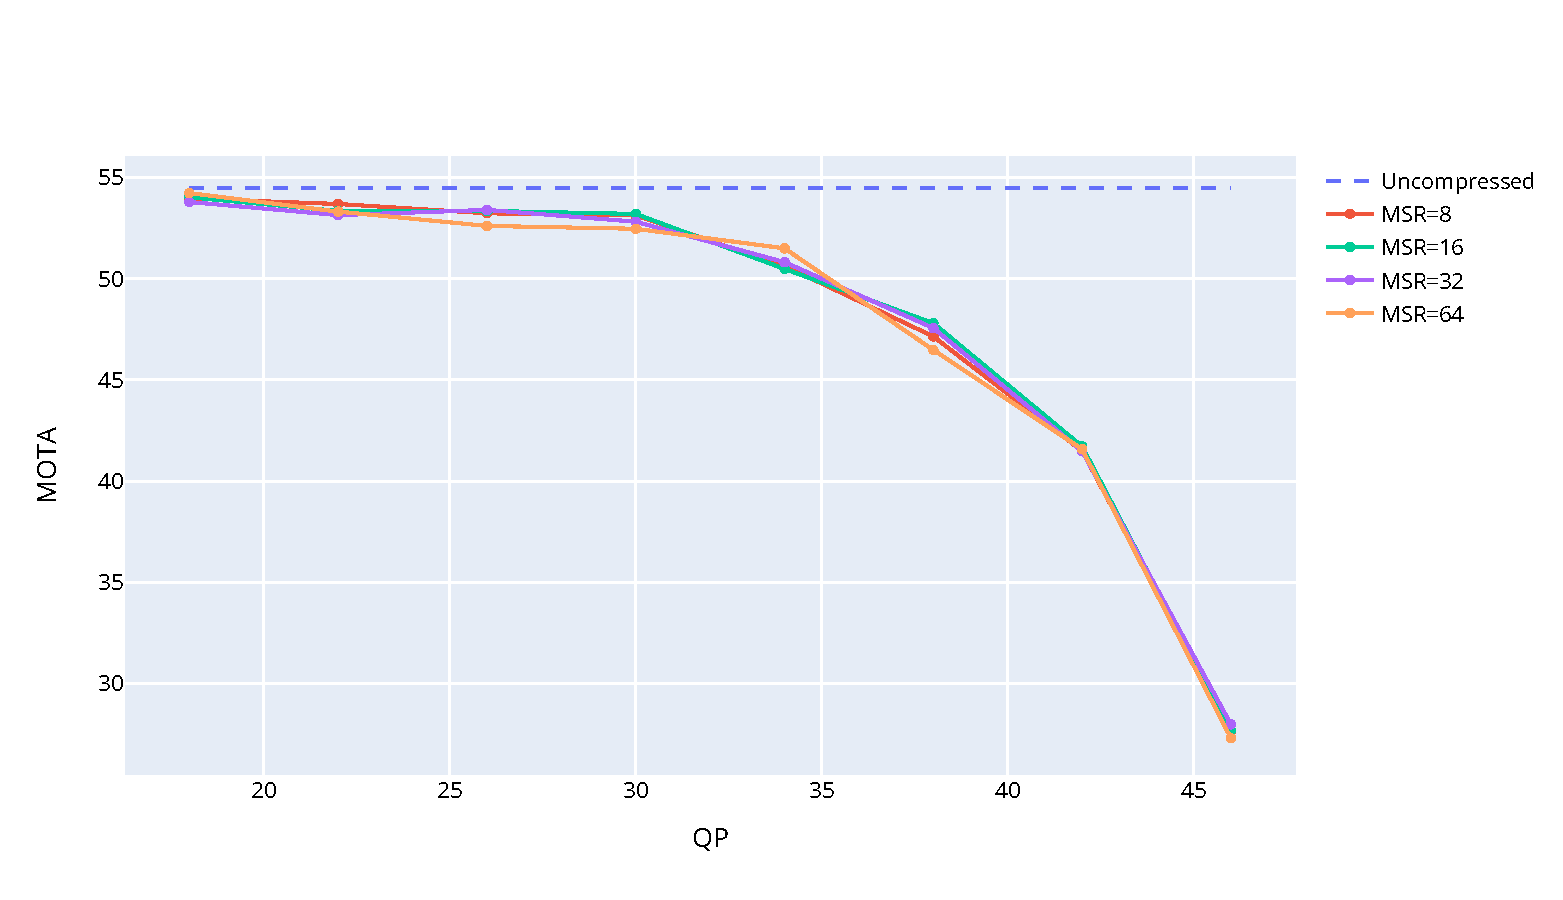
\includegraphics[width=1.0\linewidth]{img/averaged_result_all.pdf}
  \caption[Averaged Result of All Video Samples with All Object Classes]{
    
  }
  \label{fig:averaged_result_all}
\end{figure}
As you can see from the plot, the uncompressed video sequences achieved the highest performance of MOTA score. For the compressed sequences, MOTA score is lower than the uncompressed result and the higher the QP, the lower the MOTA score. Not only MOTA, we observed that the performance score of most of the metrics decrease as QP increases except IDP, Precision, and MOTP. According to the hypothesis stated in Chapter \ref{chap:background/section_e}, the higher the QP, the lower the bitrate and pixel rate, so we expected the tracking performance to be lower, and our QP result from the most metrics are consistent with the hypothesis. However, for the MSR, we do not see significant differences. To show the significant impact of QP and MSR on the each metrics score, we conducted a regression analysis. Since we have 2 independent variable
 